\section{Capacity expansion - What is the problem?}

In electricity markets, demand varies from hour to hour and as it is not storable, demand has to be met at any time of the day. If capacities are a binding constraint, there has to be rationing by rising prices. Of course, such rationing causes Welfare to decrease. On the other hand however, there are capacity costs. The literature on peak load pricing provides results on how to balance these two effects optimally. Under perfect competition, Prices will equal marginal costs in low demand periods $v=p$ (variable costs = price) and marginal costs plus a scarity rent in high demand periods. Under the assumption that there are fixed capacity costs $(c)$ how much capacity $(K)$ should be built taking into account that demand is not always high and there is a chance of $\pi$ to have high demand. The premium of the market price over marginal costs in peak periods multiplied with the chance of actually having a period of high demand reflects the value of increasing capacity by one unit $((p^p-v)*\pi)$. (In off peak periods, the corresponding premium equals zero, reflecting the fact that in such states capacity is of no value.) This value of increasing capacity by one unit must equal capacity costs per unit $((p^p-v)*\pi)=(c)$ if this condition is met, social surplus is maximised and costs are minimised. A profit maximising firm under perfect competition would invest until exactly this condition is satisfied. So under perfect competition, one could rely on the market to provide optimal incentives for capacity investments.

\begin{figure}[h]
\centering
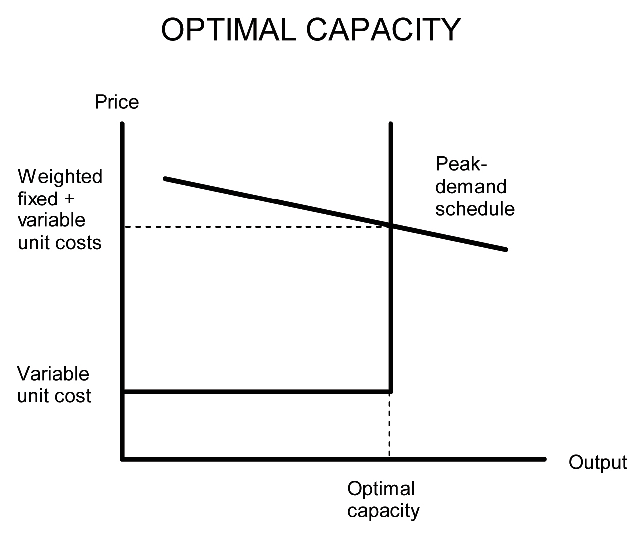
\includegraphics[width=.7\textwidth]{capacity/peak_load_opt}
      \label{von der Fehr and Harbord 1997}            
\end{figure}

If there is market power e.g. in the situation of an oligopoly this is not necessarily the case as prices which are distorted upwards may induce overinvestments. The situation of too high prices is depicted in figure two. 

\begin{figure}[h]
\centering
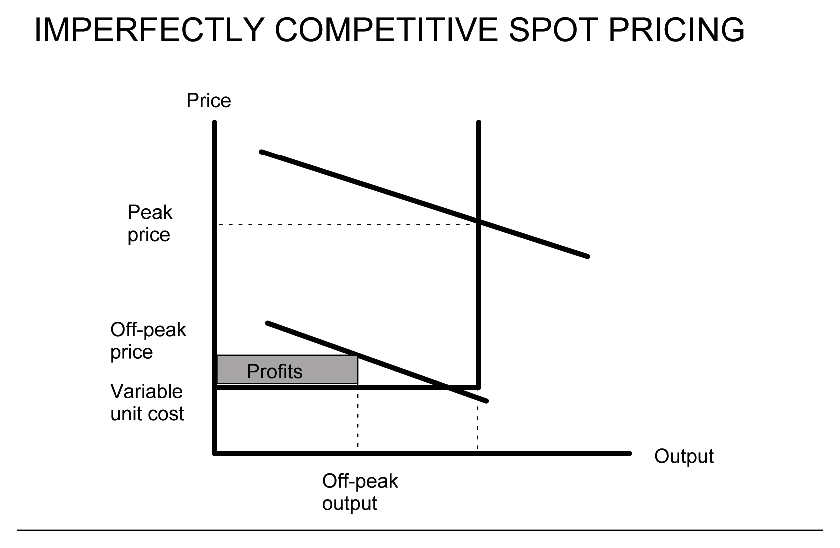
\includegraphics[width=.7\textwidth]{capacity/peak_load_toohigh}

      \label{von der Fehr and Harbord 1997}            
\end{figure}

On the other side however, firms might have an incentive to cut on investments, thereby driving up the price in peak periods and increasing their profits. This, of course would only work if there are barriers to entry beyond the unit costs of investment which are $(c)$. This can be seen in the next figure.

\begin{figure}[h]
\centering
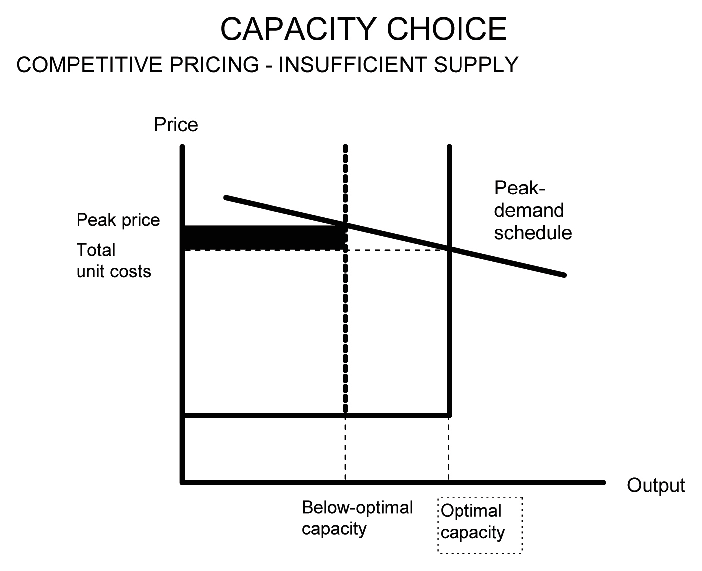
\includegraphics[width=.7\textwidth]{capacity/peak_load_insufficient}

      \label{von der Fehr and Harbord 1997}            
\end{figure}

While the socially optimal incentive to invest is still the same as above, a firm gets the following expected revenue per unit of investment:

\begin{equation}
	1/2 (1-\pi) (p^{op}-v) + \pi (w^p(K)+\frac{\partial w^p(K^*)}{\partial q}-v) - c
\end{equation}

The first part of the equation stands for possible gains of the investment that might occur during low peak periods. For simplicity we assume that there is a duopoly and a probability of $1/2$ for a new unit of capacity to be utilised. This is then multiplied by the probability to not have a peak period and the oligopoly price minus variable costs. In such periods it is possible to steal business, you would normally not have, from another firm. Such an effect can create an additional incentive to invest in capacity. As we shall see later on, this effect can be called a strategic effect of investments as well.

The second part of the equation stands for what the investing firm gains during peak periods. This equation is essentially the same as before, apart from the term ($w^{\acute{c}}$) which measures the reduction in the peak price which is due to the decreased scarity of capacity. This effect has to be taken into account now, as we switched from perfect competition to oligopoly.

So if the loss firms expect due to losses in the peak load market price are bigger than the gains due to more market share in off peak periods firms will underinvest as their incentive to invest is smaller than the optimal level under perfect competition. Of course, if the effect doe to business stealing is higher, firms will overinvest. As we shall see later on, in a two stage game such changes can be accounted for in different ways which has an effect on the predictions made.

